\section{Evaluation Details}
\label{sec:k2-post-train-eval-details}

\paragraph{Coding Tasks.}{
We evaluate Kimi-K2-Instruct's capabilities on competitive coding benchmarks, LiveCodeBench and OJBench, where Kimi-K2-Instruct attains superior performance with scores of 53.7\% and 27.1\%, respectively. This excellence spans both medium-level coding challenges, such as LeetCode and AtCoder, and hard-level contests like NOI and ICPC, outperforming leading open-source and proprietary models.
For multilingual programming proficiency, we employ MultiPL-E, covering languages including C++, C\#, Java, JavaScript, PHP, Go, Kimi-K2-Instruct surpasses top open-source models with an accuracy of 85.7\%, compared with 83.1\% for DeepSeek-V3-0324 and 78.2\% for Qwen3-235B-A22B.
In software engineering tasks, Kimi-K2-Instruct demonstrates robust performance on SWE-bench Verified (Python), SWE-lancer (Python), SWE-bench Multilingual, and Multi-SWE-bench datasets. It significantly outperforms open-source counterparts in resolving real-world code repository issues and notably narrows the performance gap with proprietary models. For example:
\begin{itemize}
    \item SWE-bench Verified (multiple attempts): 71.6\% (Kimi-K2-Instruct) vs. 80.2\% (Claude 4 Sonnet) 
    \item SWE-bench Multilingual: 47.3\% (Kimi-K2-Instruct) vs. 51.0\% (Claude 4 Sonnet)  
    \item SWE-lancer: 39.1\% (Kimi-K2-Instruct) vs. 40.8\% (Claude 4 Sonnet)  
\end{itemize}
On PaperBench, Kimi-K2-Instruct achieves an accuracy of 27.8\%, closely matching GPT-4.1 and outperforming DeepSeek-V3-0324 (12.2\%) and Qwen3-235B-A22B (8.2\%) by a substantial margin.
In terminal interaction tasks measured by TerminalBench, Kimi-K2-Instruct attains 25.0\% using the default Terminus framework and rises to 30\% within Moonshot's in-house agentic framework, underscoring its capabilities in real-world agentic programming scenarios.
Moreover, on the Aider-Polyglot benchmark, Kimi-K2-Instruct attains a 60.0\% accuracy while employing rigorous decontamination procedures, further illustrating its strength and reliability across diverse coding environments.
}

\paragraph{Tool Use Tasks.}
We evaluate multi-turn tool use with two complementary suites: $\tau^2$-Bench and ACEBench. $\tau^2$-Bench  extends the original $\tau$-bench single-control setup to a \emph{dual-control} environment in which both the agent and an LLM-simulated user have constrained tool affordances over a shared state, adding a realistic Telecom troubleshooting domain alongside the prior Airline/Retail TAU tasks and enabling analysis of coordination vs. pure reasoning. ACEBench is a large bilingual (En/Zh) API-grounded benchmark (4.5K APIs across 8 domains; 2K annotated eval items) partitioned into \textsc{Normal} (basic/personalized/atomic), \textsc{Special} (imperfect or out-of-scope inputs), and \textsc{Agent} (scenario-driven multi-turn, multi-step sandbox) tracks with automated grading of calls and outcomes. All models run in non-thinking mode; we set the temperature to 0.0, use deterministic tool adapters, score $\tau^2$ Airline/Retail/Telecom under Avg@4 seeds with Pass@1/4, and report overall on ACEBench English. Kimi-K2-Instruct averages {66.1} micro Pass@1 across $\tau^2$ vs DeepSeek-V3-0324 {48.8} / Qwen3-235B-A22B {37.3}. On ACEBench Overall Kimi-K2-Instruct scores {76.5} vs DeepSeek 72.7 / Qwen 70.5 and remains competitive with GPT-4.1 (80.1). 

\paragraph{Math \& STEM \& Logical Tasks.}
{For Math tasks, Kimi-K2-Instruct achieves consistently strong performance, averaging over Geimini-2.5-Flash by 5.3 percentage points, over DeepSeek-V3-0324 by 5.5 points and over GPT4.1 by 15.8 points. For example, on AIME 2024, Kimi-K2-Instruct scores 69.6\%, outperforming another two top open-source models by a large margin, DeepSeek-V3-0324 by 10.2 points and Qwen3-235B-A22B by 29.5 points. In STEM evaluations, Kimi-K2-Instruct achieves 75.1\% on GPQA-Diamond, outperforming DeepSeek-V3-0324 (68.4\%) and all non-thinking baselines by at least 5 percentage points. On SuperGPQA, it also exceeds the previous best open-source model, DeepSeek-V3-0324, by 3.5 points. Kimi-K2-Instruct also surpasses the other two leading models in logical reasoning. It achieves 89.0\% on ZebraLogic and 89.5\% on AutoLogi, exceeding DeepSeek-V3-0324 (84.0\%, 88.9\%) and substantially outperforming Qwen3-235B-A22B (37.7\%, 83.3\%). 

}

\paragraph{General Tasks.}
Kimi-K2-Instruct ties DeepSeek-V3-0324 on MMLU and MMLU-Pro, and takes the lead on MMLU-Redux with a 92.7 EM score—slightly ahead of GPT-4.1 (92.4) and just 1.5 points behind Claude-Opus-4. 
Beyond multiple-choice tasks, the model achieves 31.0\% accuracy on the short-answer SimpleQA—3.3 points above DeepSeek-V3-0324 and more than twice that of Qwen3-235B-A22B—though still below GPT-4.1 (42.3\%). On the adversarial free-response LiveBench (2024-11-25 snapshot), it reaches 76.4\%, surpassing Claude-Sonnet 4 (74.8\%) and leading Gemini 2.5 Flash Preview by 8.6 points. Across this challenging triad measuring breadth, depth, and robustness of world knowledge, Kimi-K2-Instruct secures a top-tier position among open-source models.
We evaluate instruction-following with IFEval and Multi-Challenge. On IFEval, Kimi-K2-Instruct scores 89.8\%, higher than DeepSeek-V3-0324 (81.1\%) and GPT-4.1 (88.0\%). On Multi-Challenge, which involves multi-turn dialogues with conflicting instructions, it achieves 54.1\%, outperforming DeepSeek-V3-0324 (31.4\%), GPT-4.1 (36.4\%), and Claude-Opus-4 (49.0\%).
These results demonstrate that Kimi-K2-Instruct integrates strong factual knowledge with consistent instruction adherence across both single- and multi-turn settings, supporting robust and reliable real-world deployment.


\paragraph{Long Context and Factuality Tasks.}



To evaluate the factuality of Kimi-K2-Instruct, we employ three benchmarks: FACTS Grounding, which measures adherence to provided documents using the proprietary models GPT-4o, Gemini 1.5 Pro and Claude 3.5 Sonnet; HHEM, which assesses summarization quality via the open-source HHEM-2.1-Open judge; and FaithJudge, which analyzes faithfulness in RAG tasks with o3-mini as the judge. Kimi-K2-Instruct scores 88.5 on FACTS Grounding, substantially outperforming all open-source rivals and even surpassing the closed-source Gemini 2.5 Flash. With HHEM-2.1-Open it achieves a hallucination rate of 1.1 \%, reported in the tables as 1 minus the rate, i.e. 98.9. On FaithJudge's RAG tasks the hallucination rate is 7.4 \%, likewise present as 92.6 for table consistency.
For long-context capabilities, Kimi-K2-Instruct outperforms all open source and proprietary models on DROP (93.5\%), and exceeds DeepSeek-V3-0324 on retrieval task MRCR (55.0\% vs 50.8\%).  
For long-context reasoning tasks FRAMES and LongBench v2, Kimi-K2-Instruct (77.1\%, 49.1\%) lags slightly behind DeepSeek-V3-0324 by around 2\%.


\paragraph{Open-Ended Evaluation}
Beyond static, closed-ended benchmarks, we evaluate the model's performance on open-ended, nuanced tasks that more closely resemble real-world usage. 

For English scenarios, we leverage the Arena-Hard-Auto v2.0 benchmark, which use LLM-as-a-judge protocols to assess generation quality across diverse, open-ended prompts~\citep{li2024crowdsourced}. These evaluations cover a wide range of high-difficulty prompts and are widely recognized in the research community. 
On Arena-Hard-Auto v2.0, Kimi-K2-Instruct achieves state-of-the-art win-rate on both hard prompts (54.5\%) and creative writing tasks (85.0\%), outperforming all open-source models and rivaling top proprietary systems such as GPT-4.1 and Claude Sonnet. These results underscore the model's strength in handling complex reasoning and nuanced generation under diverse, unconstrained settings.


However, Arena-Hard-Auto provides limited coverage of Chinese-specific tasks. To address this gap, we developed an in-house held-out benchmark grounded in authentic user queries. 
To safeguard the integrity of the evaluation, the benchmark data is access-restricted, thereby eliminating the risk of overfitting.

As shown in Figure~\ref{fig:posttrain_inhouse_eval}, Kimi-K2-Instruct shows strong performance across all comparisons on Chinese in-house benchmarks. It outperforms ChatGPT-4o-latest with a 65.4\% win rate, Claude Sonnet 4 with 64.6\%, and DeepSeek-V3-0324 with 59.6\%.
In all cases, the loss rate stays low (around 17\%), indicating that Kimi-K2-Instruct rarely falls behind. The high win rates and consistent margins demonstrate its strong ability on open-ended Chinese tasks.

In addition to controlled evaluations, we also consider real-world user preference through public human assessments. As of July 17, 2025, Kimi-K2-Instruct ranked as the top open-source model and fifth overall on the LMSYS Arena leaderboard\footnote{\url{https://lmarena.ai/leaderboard/text}}, based on over 3,000 blind votes from real users. Unlike LLM-as-a-judge protocols, this leaderboard reflects direct human preference on diverse, user-submitted prompts, providing a complementary perspective on practical model performance.

The results on Arena-Hard-Auto, our in-house benchmark and votes from LMSYS Arena collectively offer a comprehensive view of Kimi-K2-Instruct's open-ended capabilities, showing that it is a highly preferred model in real-world user experience across English and Chinese.


\begin{figure}
    \centering
    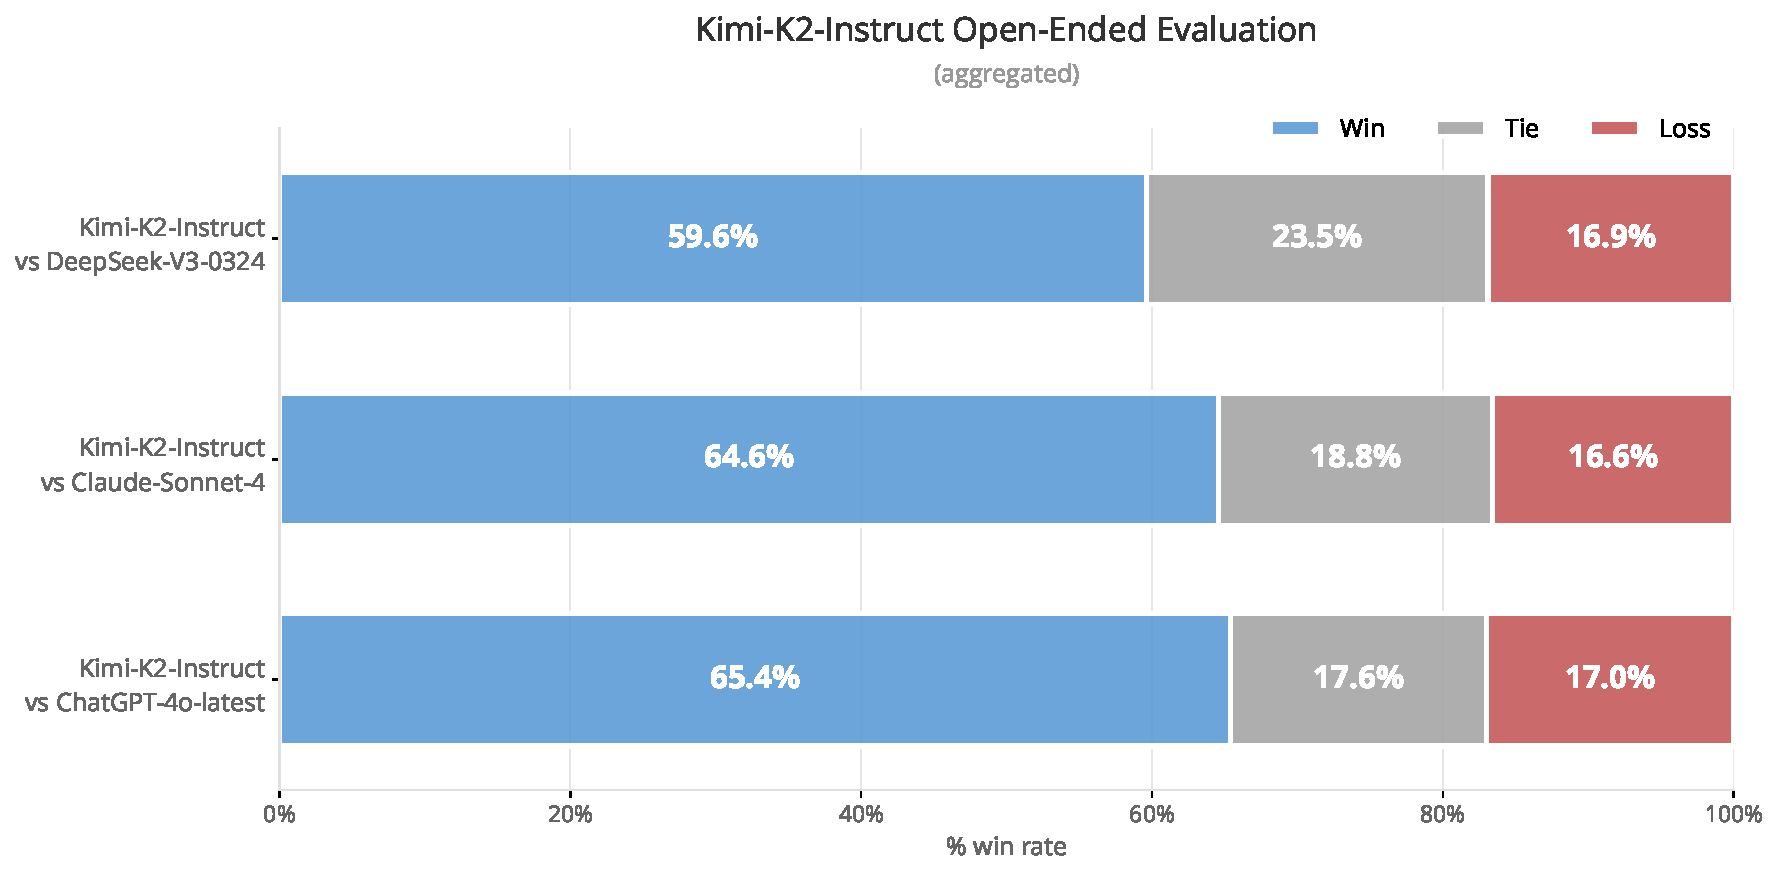
\includegraphics[width=0.8\linewidth]{figures/posttrain_inhouse_eval.pdf}
    \caption{Chinese in-house benchmark evaluation.}
    \label{fig:posttrain_inhouse_eval}
\end{figure}

